\documentclass{article}
\usepackage[utf8]{inputenc}
\usepackage{indentfirst}
\usepackage{amsmath}
\usepackage{amssymb}
\usepackage{graphicx}
\usepackage{appendix}
\usepackage{subcaption}
\usepackage{hyperref}
%\usepackage{wrapfig}

\begin{document}
\title{Development of Neural Networks for Learning The Boltzmann Equation	 }
\author{Thomas V Nguyen}
\maketitle
\begin{center}
Department of Mathematics, CSUN, Northridge, CA 91303 \\
Advisor: Professor Alexander M. Alekseenko
\end{center}
\section*{Abstract} During the past decades, there are different methods that have been developed to solve the Boltzmann equation: the direct simulation Monte Carlo (DSMC) method, the lattice Boltzmann method (LBM), and the direct deterministic method for computing the Boltzmann equation. In this paper, we explore the physical aspect of the Boltzmann equation and the novel neural network methods for learning the solutions of the Boltzmann equation.
\section{Introduction} \label{Intro}
The Boltzmann equation describes the statistical behavior of a system of rarefied gases in the non-equilibrium, nonlinear state. The equation analyzes a probability distribution $f(t,\vec{x}, \vec{v})$ for the position and velocity of a typical particle in the small region of $d^3x$ and a small region $d^3v$ of velocity space. The Boltzmann equation is a nonlinear integral differential equation and the unknown function in the equation is a probability density function $f(t,\vec{x}, \vec{v})$ in six-dimensional space of a particle position and velocity and the function $f(t,\vec{x}, \vec{v})$ is evolved in time t. Exact solutions to the Boltzmann equations have been difficult to obtain and is not generally usable in practical problems until the advent of computer technology and numerical analysis methods. Numerically, there have been two development methods of simulating and solving the Boltzmann equation: stochastic and deterministic methods. 

For the stochastic methods, the direct simulation Monte (DSMC) method has been widely used. The DSMC method was first introduced by G.A. Bird in 1963 \cite{BirdGA1} and have been a popular method for numerical simulation of rarefied gas flows. This method randomly generates the number of simulated particles and tracking the binary collisions among the simulated particles such that to reproduce the underlying physics of the Boltzmann equation. The popular of the DSMC is due to the combination of accuracy, simplicity, and computational efficiency. Beside the Bird’s original method, There are different implementations of DSMC method have developed as described in \cite{DSMC1, DSMC2, DSMC3}. 

The deterministic method of solving the Boltzmann equation is suitable for parallel processing for the computer system that have many CPU cores. One of the deterministic method of solving the Boltzmann equation is the Lattice-Boltzmann method (LBM )as described in the \cite{LBM1, LBM2}. The objective of the LBM methods is to provide simpler model equations for rarefied gas dynamics. Another deterministic method of solving Boltzmann equation is called the discontinuous Galerkin (DG) velocity approximations that can accommodate for the functions discontinuities. \cite{Alekseenko1, Alekseenko2} explored the high order DG discretization using the Gauss quadrature nodes and the Lagrange polynomial basis functions. \cite{Alekseenko4} used the Discrete Fourier Transform to compute the DG approximation for the Boltzmann solution. One can refer \cite{VVAristo} to study the different direct methods for solving the Boltzmann Equation.

In this paper, we will develop a novel method by applying the machine learning and neural networks methodologies to learn the solutions of Boltzmann equation. Specifically, we use the autoencoder to reduce the dimensions of  input layers to a much lower dimensions in the hidden layers called coding layers so that we can learn the essential features of the solutions. The autoencoder's inputs are the solutions of the Boltzmann equation and the autoencoder's outputs are the predicted solutions the Boltzmann equation. The hidden layers' inputs have the reduced dimension comparing with the autoencoder input dimension. This paper is orgarnized as follow:
\begin{itemize}
	\item Section 2 describes the gas kinetic assumptions and the brief derivation of the Boltzmann equation and its applications.
	\item Section 3 describes the deterministic method for obtaining the solutions of the Boltzmann equation as discussed in \cite{Alekseenko2, Alekseenko4} and the structure of the solution data. This solution data is used as the dataset for neural networks' input.
	\item Section 4 describes the general neural network architecture and specifically how the autoencoder is used to reduce the input dimension of the Boltzmann equation solutions and how the hidden layers use the reduced dimension data to predict the outputs which are the approximations of the autoencoder input.
	\item Section 5 compares the computational efficiency between the deterministic method and the autoencoder method for the solutions of Boltzmann equation.
\end{itemize}

\section{The Boltzmann Equation and its application}
In this section, we briefly describe the derivation of the Boltzmann equation so that we can grasp the physical meaning of the Boltzmann equation. One can check \cite{RarefiedGasD, IntroBoltz} for the detail of derivation of the Boltzmann equation.
\subsection{The rarefied gas assumptions}
The Boltzmann equation is derived with the following assumptions of the kinetic theory of gases:
\begin{itemize}
\item Gas consists of very small particles known as molecules having the same mass.
\item The motion of the molecules can be described by Newtonian mechanics.
\item The number of molecules is so large that statistics can be applied.	content...
\item The total volume of the individual gas molecules added up is negligible compared to the volume of the container. Hence, only binary collisions occur between molecules and collisions are perfectly elastic. Kinetic energy and momentum are conserved.
\item The elapsed time of a collision between a molecule and the container's wall is negligible when compared to the time between successive collisions.
\end{itemize}
\subsection{The Boltzmann equation} \label{BoltzEq}
The Boltzmann equation analyzes a probability distribution $f(t, \vec{x}, \vec{v})$ of a particle in a small cell of $(\vec{x}, \vec{v})=(x,y,z,v_x,v_y,v_z)$ evolves with time $t$ in a non-equilibrium state. Suppose at time $t$, particles are in a cell $(\vec{x},\vec{v})$. If an external force $\vec{\textbf{F}}$ instantly acts on each particle causing particles changing in position after $\Delta t$, we have 
\begin{equation} \label{BoltzEqGeneral}
\frac{\partial f}{\partial t} + \vec{v}\cdot\nabla_{\vec{x}}f + \frac{\vec{\textbf{F}}}{m}\cdot\nabla_{\vec{x}}f = \left(\frac{\partial f}{\partial t}\right)_{collision} = I[f](t,\vec{x},\vec{v})
\end{equation}
If there is no external force $\vec{\textbf{F}} = 0$, then (1) is written as:
\begin{equation} \label{BoltzEqNoForce}
\frac{\partial f}{\partial t} + \vec{v}\cdot\nabla_{\vec{x}}f = I[f](t,\vec{x},\vec{v})
\end{equation}
Here $I[f](t,\vec{x},\vec{v})$ is the molecular collision operator. For binary collisions between molecules, the collision operator takes the form:
\begin{multline} \label{CollOp}
I[f](t,\vec{x},\vec{v}) = \\ \int_{\mathbb{R}^3}\int_{\mathbb{S}^2}(f(t,\vec{x},\vec{v}^\prime)f(t,\vec{x},\vec{u}^\prime) - f(t,\vec{x},\vec{v})f(t,\vec{x},\vec{u}))B(|g|,\cos\theta)d\sigma d\vec{u}
\end{multline}
Where
\begin{itemize}
	\item $\vec{v}$ and $\vec{u}$ are the pre-collision velocities of a pair of molecules.
	\item $\vec{g} = \vec{v} - \vec{u}$.
	\item $\mathbb{S}^2$ is a unit sphere in $\mathbb{R}^3$ centered at the origin.
	\item $\vec{w}$ is the unit vector connecting the origin and a point on $\mathbb{S}^2$.
	\item $\theta$ is the deflection angle defined by the equation $\cos\theta = \vec{w}\cdot\vec{g}/|g|$.
	\item $d\theta = sin\theta d\theta d\varepsilon$ where $\varepsilon$ is the azimuthal angle parametrizes $\vec{w}$ together with the angle $\theta$.
	\item $\vec{v}$ and $\vec{u}$ are the post-collision velocities of a pair of particles and are computed by
	\begin{equation*}
		\vec{v}^\prime = \vec{v} - \frac{1}{2}(\vec{g} - |g|\vec{w}), \quad \vec{u}^\prime = \vec{v} - \frac{1}{2}(\vec{g} - |g|\vec{w})
	\end{equation*}
	\item The kernel $B(|g|,\cos\theta)$ characterizes interactions of the molecules and is selected appropriately to reproduce the desired characteristics of the gas.
\end{itemize}

For the spatially homogeneous relaxation problem, we assume that the distribution density function of molecular velocities $f(t, \vec{x}, \vec{v})$ is constant in the spatial variable $\vec{x}$, i.e., $f(t, \vec{x}, \vec{v}) = f(t, \vec{v})$. Then the derivative of solution with respect to $\vec{x}$ vanishes and the spatially homogeneous form of the Boltzmann equation is:
\begin{equation}	\label{BoltzHomo}
	\frac{\partial}{\partial t}f(t,\vec{v}) = I[f](t, \vec{v})
\end{equation}
\subsection{The Boltzmann equation's applications}
Below are the applications of the Boltzmann equation:
\begin{itemize}
	\item The Boltzmann equation is a foundation for deriving the theory of thermodynamics and kinetic theory of gasses.
	\item The Boltzmann equation can be used to determine how physical quantities change, such as heat energy and momentum, when a fluid is in transport. One may also derive other properties characteristic to fluids such as thermal.
	\item In the advent of hypersonic flight, flows in satellite electric propulsion thrusters and around thrusters, and in re-entry from space flight, the Boltzmann equation can be used to describe accurately for these aerodynamics flights in rarefied gas regimes.
\end{itemize}

\section{Deterministic Numerical solutions for the Boltzmann equation and the solution data set} \label{BoltzSol}
In this section, we will briefly describe the numerical methods of obtaining the solutions of the Boltzmann equation. One can refer to \cite{Alekseenko2, Alekseenko4} for the detail of these methods. We will then describe the solution data set obtained by these two numerical methods. The solution data set will be used in section \ref{NN} for learning the solutions of Boltzmann equation.
\subsection{Deterministic solution of the spatially homogeneous Boltzmann equation using discontinuous Galerkin discritization in the velocity space} 
To evaluate the collision operator in equation (\ref{BoltzHomo}), as described in \cite{Alekseenko2}, we select a rectangular parallelepiped in the velocity space  and partition this region into parallelepipeds $K_j$. Let $\vec{v} = (u,v,w)$ and let $s_u, s_v, s_w$ be the degrees of the polynomial basis functions in the velocity components $u, v$ and $w$ respectively. Let $K_j = [u^L_j, u^R_j]\times[v^L_j,v^R_j]\times[w^L_j,w^R_j]$. We construct the Lagrange basis functions as follows:

We introduce the nodes of Gauss quadratures of orders $s_u, s_v$ and $s_w$ on each of the intervals $[u^L_j,u^R_j], [v^L_j,v^R_j]$ and $[w^L_j, w^R_j]$ respectively. Let these nodes be denoted $\kappa^u_{p;j}, p=1,\dots,s_u, \kappa^v_{q;j} q=1,\dots,s_v$ and $\kappa^w_{r;j}, r=1,\dots,s_w$. Then the Lagrange basis functions are defined as:
\begin{equation*}
\phi^u_{l;j} = \prod_{\substack{p=1,s^u \\ p \neq l}}\frac{\kappa^u_{p;j} - u}{\kappa^u_{p;j} - \kappa^u_{l;j}}, \quad \phi^v_{m;j} = \prod_{\substack{q=1,s^v \\ 1 \neq m}}\frac{\kappa^v_{q;j} - u}{\kappa^v_{q;j} - \kappa^v_{m;j}}, \quad \phi^w_{r;j} = \prod_{\substack{r=1,s^w \\ p \neq n}}\frac{\kappa^w_{r;j} - w}{\kappa^w_{r;j} - \kappa^w_{n;j}}
\end{equation*}
The three-dimensional basis functions are given as
\begin{equation}
	\phi_{i;j}(\vec{v})= \phi^u_{l;j}(u)\phi^v_{m;j}(v)\phi^w_{n;j}(w)
\end{equation} 
Where $i = 1,\dots,s:=s_us_vs_w$ is the index running through all combinations of $l, n and m$.
The following identities hold for basis function $\phi_{i;j}(\vec{v})$:
\begin{equation}
\int_{K_j}\phi_{p;j}(\vec{v})d\vec{v}= \frac{\omega_p\Delta\vec{v}^j}{8}\delta_{pq} \quad and\quad \int_{K_j}\vec{v}\phi_{p;j}(\vec{v})d\vec{v}= \frac{w_p\Delta\vec{v}^j}{8}\vec{v}_{p;j}\delta_{pq}
\end{equation}
where indices $p$ and $q$ run over all combinations of $l, n, and m$ in three dimensional basis functions $\phi_{i;j}(\vec{v})= \phi^u_{l;j}(u)\phi^v_{m;j}(v)\phi^w_{n;j}(w)$ and the vectors $\vec{v}_{p;j}=(\kappa^u_{l;j},\kappa^v_{m;j},\kappa^w_{n;j})$. $\Delta\vec{v}^j=(u^R_j - u^L_j)(v^R_j - v^L_j)(w^R_j - w^L_j)$ and $w_i = w^{s_u}_lw^{s_v}_mw^{s_w}_n$, where $w^{s_u}_l, w^{s_v}_m and w^{s_w}_n$ are the weights of the Gauss quadratures of orders $s_u, s_v and s_w respectively.$
For each $K_i$, the solution for Boltzmann equation can be written in the nodal-DG velocity discetization as:
\begin{equation}
	f(t,\vec{x},\vec{v})|_{K_i} = \sum_{i=1s}f_{i;j}(t,\vec{x})\phi_{i,j}(\vec{v})
\end{equation}
Repeating this for all $K_j$, we can write (\ref{BoltzEqGeneral}) in the numerical form:
\begin{equation}
\partial_tf_{i;j}(t,\vec{x}) + \vec{v}_{i,j}\cdot\nabla_xf_{i,j}(t,\vec{x}) = \frac{8}{w_i\delta\vec{v}^j}I_{\phi_{i;j}}
\end{equation}
with 
\begin{equation} \label{directColl}
I_{\phi_{i;j}} = \int_{\mathbb{R}^3}\int_{\mathbb{R}^3}f(t,\vec{x},\vec{v})f(t,\vec{x},\vec{v}_1)A(\vec{v},\vec{v}_1;\phi_{i;j})d\vec{v}_1d\vec{v}
\end{equation}
where
\begin{equation} \label{kernelA}
	A(\vec{v},\vec{v}_1;\phi_{i;j}) = |g|^\alpha\int_{\mathbb{S}^2}(\phi_{i;j}(\vec{v}') - \phi_{i;j}(\vec{v}))b_\alpha d\sigma
\end{equation}
In \cite{Alekseenko1,Alekseenko2} a nodal dicontinuous Galerkin (DG) discretization of the collision operator leads to a $O(N^{\frac{8}{3}})$ operations where $N$ is the total number of discrete velocity points.
The operator $A(\vec{v},\vec{v}_1;\phi_{i;j})$ in (\ref{kernelA}) has the shift invariant property:
\begin{equation}
A(\vec{v}+\xi,\vec{v}_1+\xi;\phi_{i;j}(\vec{v}-\xi)) = A(\vec{v},\vec{v}_1;\phi_{i;j}) \quad \forall\xi \in \mathbb{R}^3
\end{equation}
With the shift invariant property, we can obtain a bilinear convolution as:
\begin{equation} \label{Convo}
I_i(\vec{\xi}) = \int_{\mathbb{R}^3}\int_{\mathbb{R}^3}f(t,\vec{x},\vec{v} - \vec{\xi})f(t,\vec{v}_1 - \vec{\xi})A(\vec{v},\vec{v}_1;\phi_{i;c})d\vec{v}d\vec{v}_1
\end{equation}
The convolution formular (\ref{Convo}) is used in \cite{Alekseenko4} to develop an $O(N^2)$ method using discrete Fourier transform.

\subsection{The Boltzmann equation's solution dataset}
In this section, we will discuss the method of generating the solution data set of the Boltzmann equation using the numerical methods described in section \ref{BoltzSol}. This solution dataset will be used in section \ref{NN} for learning the Boltzmann equation's solution. The solution data was obtained based on the spatially homogeneous equation (\ref{BoltzHomo}): $\frac{\partial}{\partial t}f(t,\vec{v}) = I[f](t, \vec{v})$. Below are the steps of generating the solution dataset:
\begin{itemize}
\item Macroparameters of two homogeneous Gaussians are randomly generated and consecutively normalized so that the sum of Gaussians has unit density, zero bulk velocity, and pre-selected values of temperature of 0.5 and 0.2. The sum of two homogeneous Gaussians is used as the initial data for the solution.
\item Equation \ref{BoltzHomo} is solved by \cite{Alekseenko4} for each set of randomly generated initial data. As the solutions are evolving in time, they are saved at even intervals of time. The computed solutions were saved in the files which will be used to construct the dataset for section \ref{NN}.
\item The solutions were computed on $41^3$ discrete points. Due to the fact that solutions are very small near the boundary, a number of discrete points can be removed from the solution for analysis. The truncated solution has $25^3$ discrete points and the dataset has about 5000  generated solution data.
 
\end{itemize}

\section{Neural network for learning the solutions of Boltzmann equation} \label{NN}
In this section, we will describe a general architecture of a neural network. How the gradient descent and backpropagation algorithms are used to train a neural network to obtain the weights of a neural network. Then we will specifically describe the autoencoder architectures that are used in this paper to learn the Boltzmann solution dataset.
\subsection{Neural networks and autoencoder architectures} \label{NN}
\subsubsection{A general fully connected neural network architecture } \label{FCNN}
A general neural network composes of an input layer, a stack of hidden layers, and an output layer as shown in figure \ref{fig:NN} which has two hidden layers. Figgure \ref{fig:NN} is called a fully connected neural network because each neuron in a hidden layer is connected to all the neurons in the previous layer.
\begin{figure}[h]
	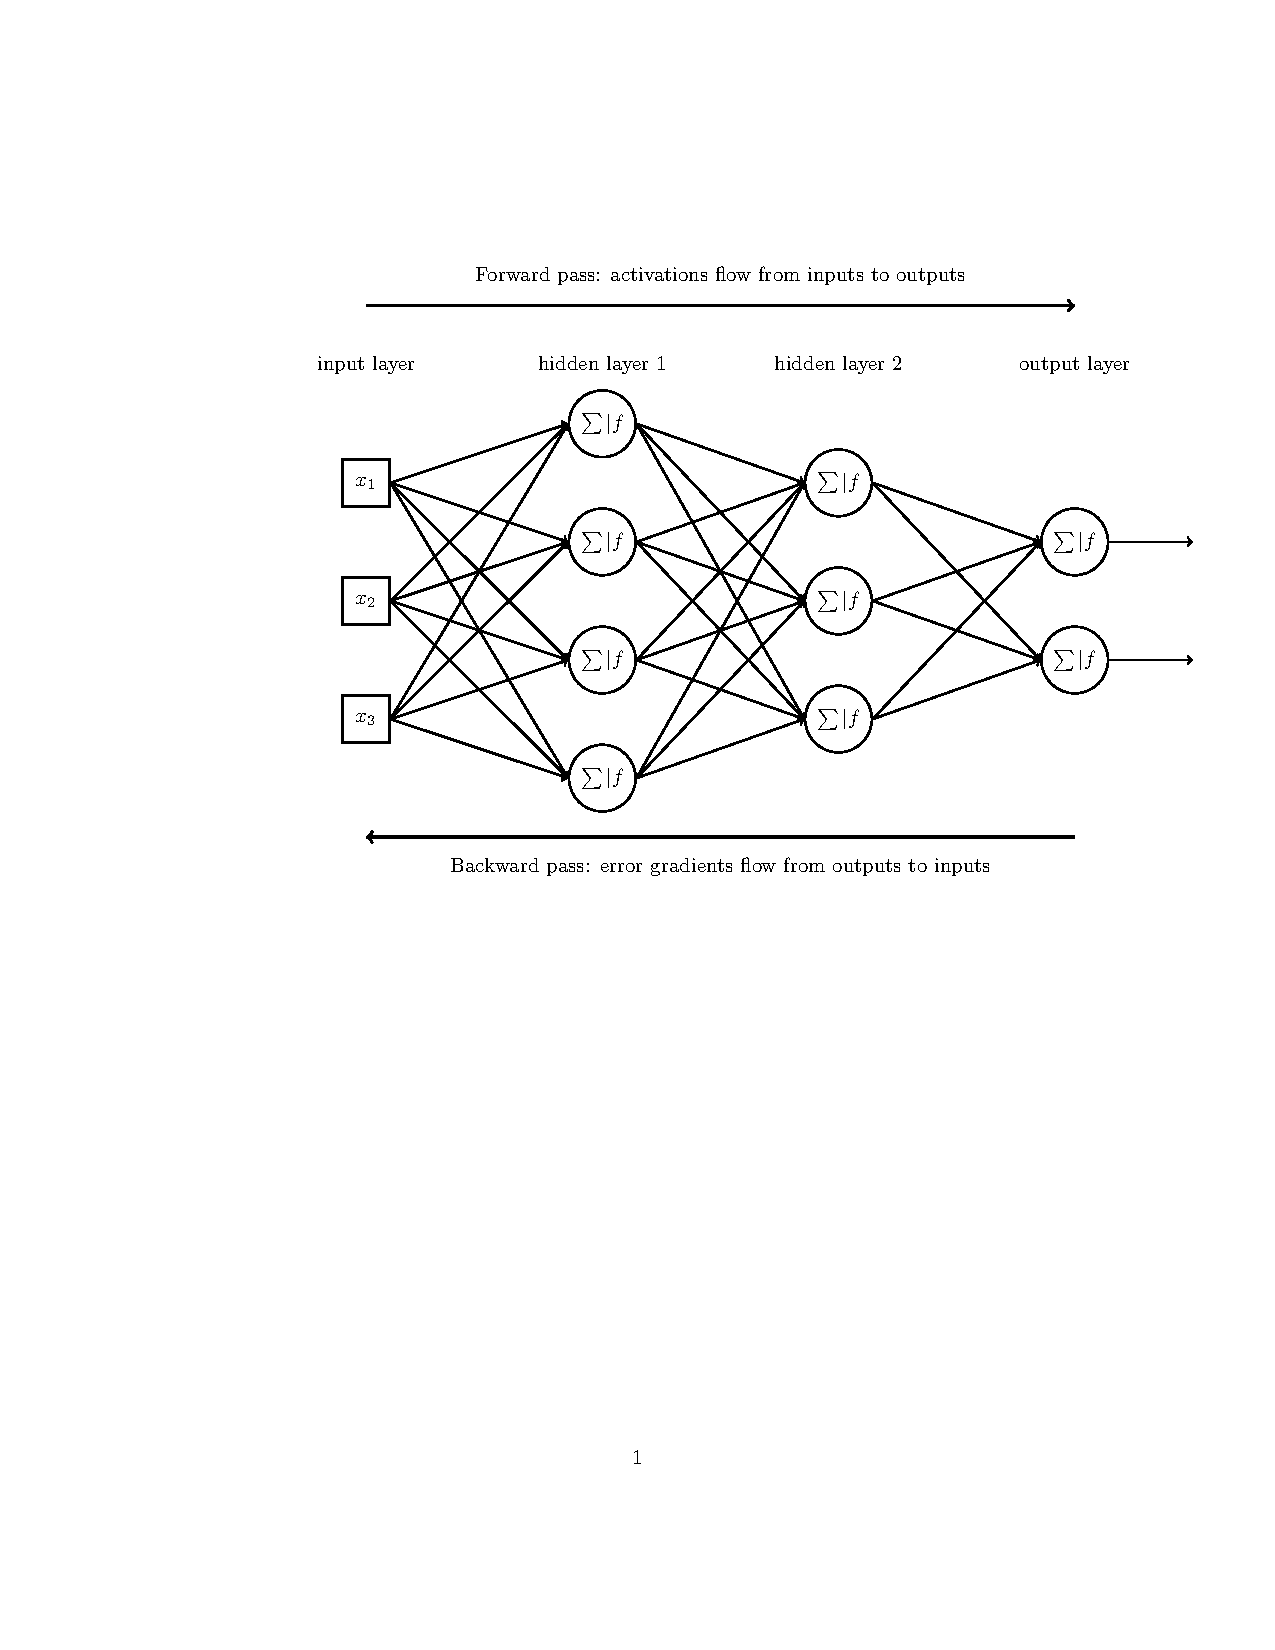
\includegraphics[width=.75\textwidth]{NN.pdf}
	\caption{A general neural network architecture}
	\label{fig:NN}
\end{figure}
A typical neural network may have many hidden layers. Each hidden layer consists of number of neuron and the outputs of each neuron are connected to the inputs of the neurons of the next layer.
The figure \ref{fig:neuron} shows the components of a neuron. 
\begin{figure}[h]
\centering
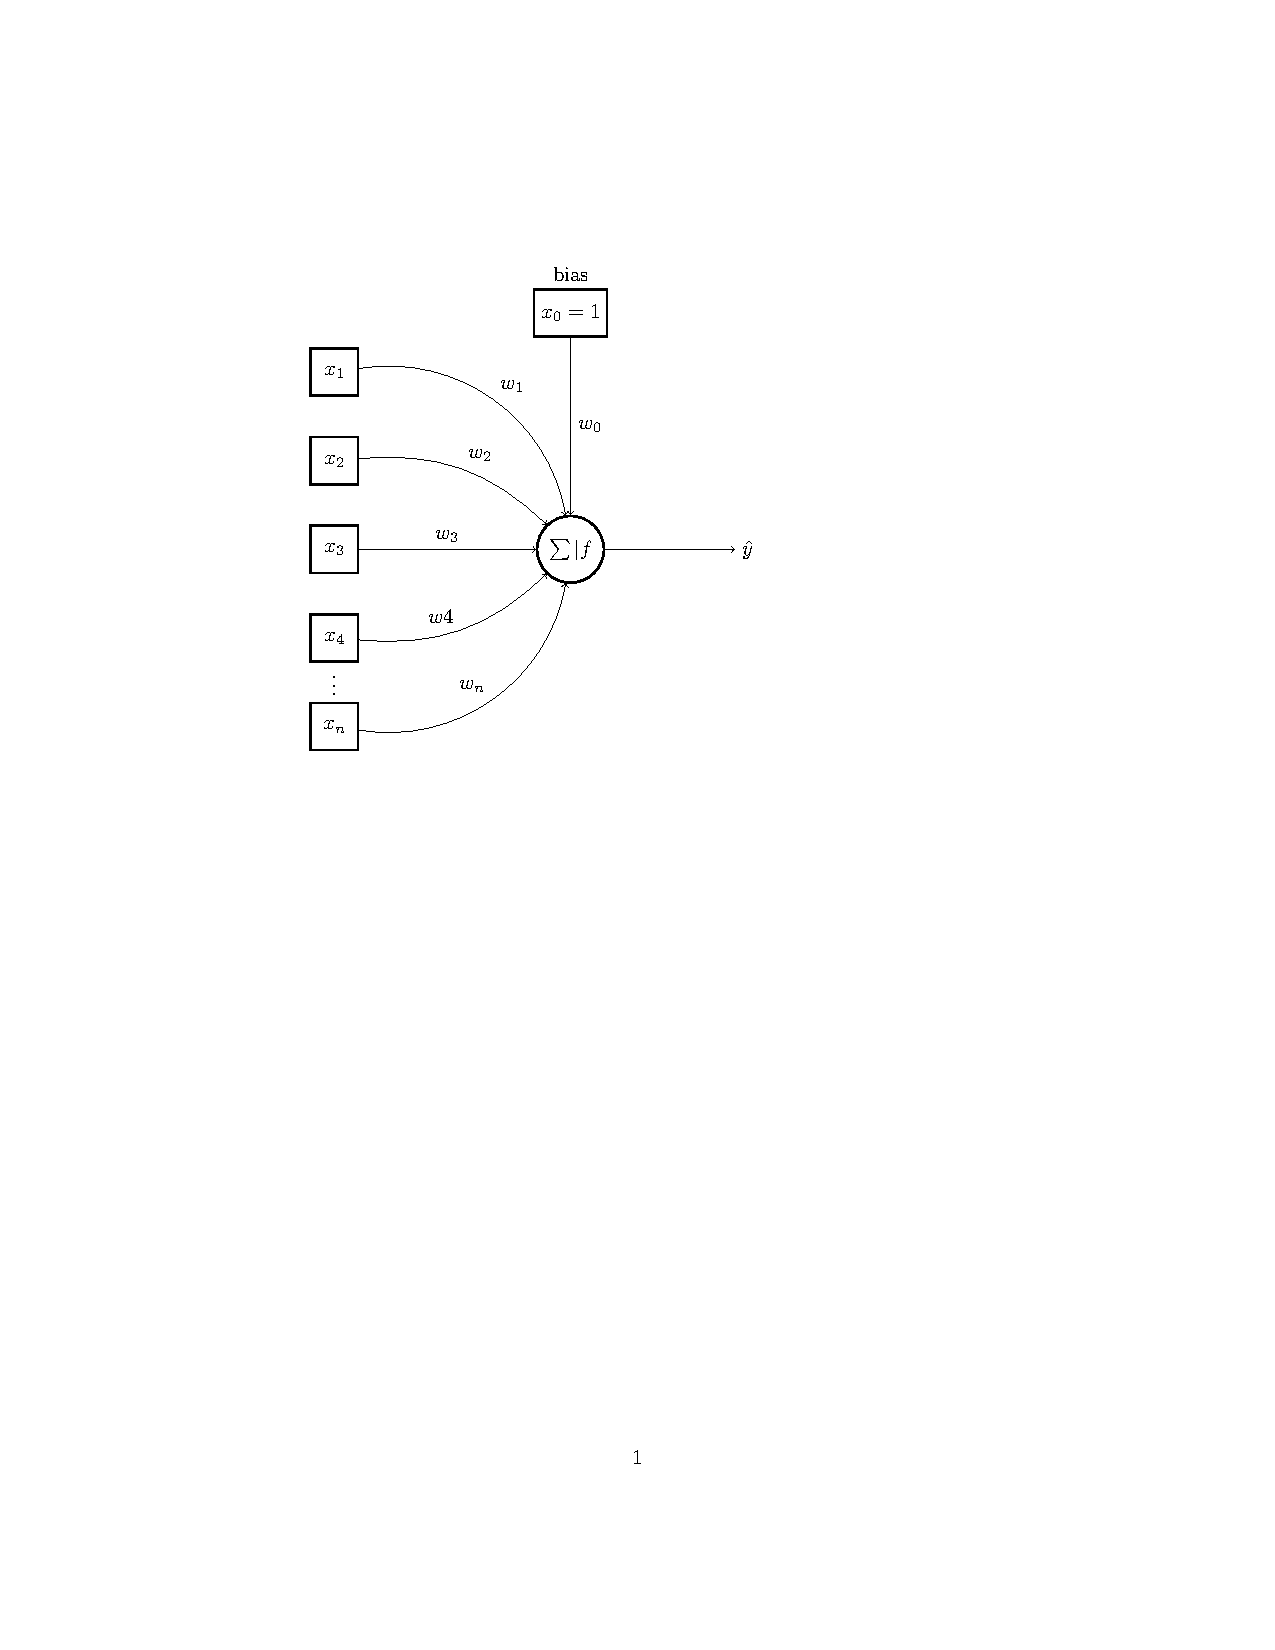
\includegraphics[width=.75\textwidth]{Neuron.pdf}	
\caption{A neurol architecture}
\label{fig:neuron}
\end{figure}

As shown in figure \ref{fig:neuron}, a neuron receives n inputs $[x_1,x_2, \dots, x_n]$. Each input $x_i$ is associated with a weight $w_i$ and the sum is computed by multiply each input $x_i$ by its associated weight $w_i$ and then sum the resulting values. The result of the weighted sum is then passed into the activation function $f$. Mathematically, we can express these calculations as:
\begin{equation} \label{neuronfunc}
\hat{y} = f\left(\sum_{i=0}^{n}x_i \times w_i\right) = f(z)
\end{equation}
Figure \ref{fig:actFuncs} shows the popular activation functions. Recently, the rectified linear unit function (ReLU) has become the default activation function due to it works well and fast to compute despite it is not differentiable at 0.
\begin{figure}[h]
\centering
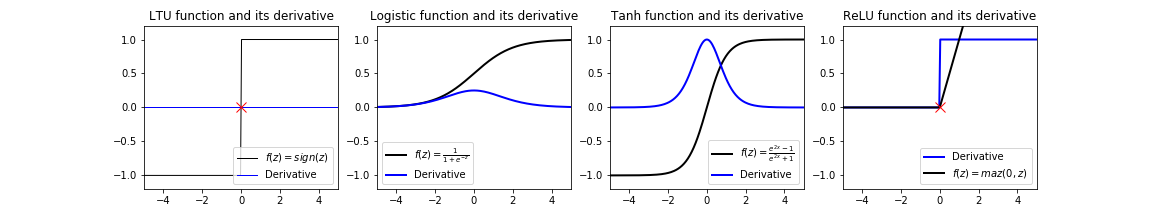
\includegraphics[width=1.0\textwidth]{activationFuncs.png}
\caption{Activation functions}
\label{fig:actFuncs}
\end{figure}
The reason that we need an activation function because each activation function is a nonlinear function and $\left(\sum_{i=0}^{n}x_i \times w_i\right)$ is a linear function. By chaining the $\left(\sum_{i=0}^{n}x_i \times w_i\right)$ to a nonlinear activation function $f$, the resulting function is a nonlinear function which can be used to fit any non-linear dataset.

To train a neuron is to obtain the set of weights $w_i$ such that the function $f(z)$ is best fit of the dataset. There are two common error functions that are used to measure the error of the expected output value $y_i$ of a sample $x_i$ and the estimated output value $\hat{y}$ returned from the model: the mean square error (MSE) function and the mean absolute error (MAE) function:
\begin{equation}
MSE = \frac{1}{m}\sum_{i=1}^{m}(\hat{y}^i - y^i)^2 
\end{equation}
\begin{equation}
MAE = \frac{1}{m}\sum_{i=1}^{m}|\hat{y}^i - y^i|
\end{equation}
where m is the number of instances in the dataset, $x^i$ is a vector of all the input features of the $i^{ih}$ instance, and $y^i$ is the expected output value. To obtain the set of weights $w_i$ that is best fit to the dataset is to find the optimal solution for either MSE or MAE functions. 

Gradient descent algorithm is the popular method to find the optimal solution any convex function like MSE or MAE error functions. The gradient descent algorithm starts with an random weight vector $\vec{\mathbf{w}}$ and measures the local gradient of the error function with respect to the parameter weight vector $\vec{\mathbf{w}}$. Then it goes in the direction of descending gradient until the error function reaches to the minimum. Specifically, for a dataset $\mathbf{X}^{m \times n}$, in each iteration, the weight vector is computed as:
\begin{equation} \label{fullbatchweightComp}
\mathbf{\vec{w}}^{t+1} = \mathbf{\vec{w}}^t - \eta\nabla_{\mathbf{\vec{w}}}MSE(\mathbf{\vec{w}}) 
\end{equation}
where $\eta$ is a learning rate hyperparameter and
\begin{equation} \label{fullbatchGrad}
\nabla_{\mathbf{\vec{w}}}MSE(\mathbf{\vec{w}})= \frac{2}{m}\mathbf{X^T}(\mathbf{X}\vec{\mathbf{w}} - \mathbf{y})
\end{equation}
The (\ref{fullbatchweightComp}) and (\ref{fullbatchGrad}) is called batch gradient descent algorithm which uses the entire training dataset to compute the gradient at every step and it is expensive. The least expensive gradient descent is used stochastic gradient descent (SGD) algorithm which randomly picks a sample in every step and computes the gradients only on that random instance. In between, there is a algorithm called mini-batch gradient descent algorithm which compute the gradients based on small random sets of instances call mini-batches. 

The above discussion is for training a neuron. A neural network is composed of an input layer, an output layer, and number of hidden layers in between the input and output layer. Each neuron in a hidden layer is fully or partially connected to the neurons in the next layer. Backpropagation algorithm is used to train a neural network. The backprogation is a two-stage process: forward pass and backward pass as shown in figure \ref{fig:NN}. Starting with random values of all the weight, below is the outline steps of the backpropagation algorithm:
\begin{enumerate}
\item The inputs are passed to the input layer which sends these inputs to the first hidden layer. The algorithm computes the outputs of all the neurons in this layer. Then the results are passed on to the next hidden layer and so on until the computed results reach to the output layer. This is a forward pass. All the intermediate results are recorded since these computed results are needed for the backward pass.
\item Using a loss function, the algorithm measures the network's output error. It then computes how much each output connection contributed to the error.
\item The algorithm then calculates error gradient for each neuron in the hidden layer below the output layer and propagating the error gradient backward to the hidden layers until the algorithm reaches to the input layer.
\item Using these gradient errors and gradient descent method, the algorithm to update all the connection weights in the network. 
\end{enumerate}
The algorithm iterates these steps until the error of the network converges to the acceptable minimum value.

\subsubsection{Convolutional neural network architecture} \label{CNN}
In this project, we also use the convolutional neural network (CNN) to learn the Boltzmann equation's solutions. As shown in \ref{fig:CNN}, a CNN consists of input layers, convolutional layers, pooling layers, fully-connected layers, activation functions, and output layers. Comparing with the fully-connected neural network, a CNN architecture introduces two new building block: convolutional layers and pooling layers. Below, we briefly describes the structure of a convolutional layer and a pooling layer.

In a convolutional layer, neurons are only partially connected with the neurons in the previous layer: each neuron is only connected to the neurons located within a small rectangle in the previous layer. This small window is called the receptive field. This architecture allows the CNN to focus on small low-level features in the preceding hidden layer, then assemble them into larger higher-level features in the next hidden layer, and so on. This receptive field window is then moved across the layer horizontally and vertically with a step size called the stride length. All the receptive field share the same set of weights known as the kernel or filter. The outputs from this filter is known as a feature map. A convolutional layer may have multiple filters with each filter has different weights allowing a convolutional layer to detect multiple features of the inputs. 

After the convolutional layer is the pooling layer which is used to subsample the input image. Just like the convolutinal layer structure, each neuron in a pooling layer is connected to a number of neurons located in a small window receptive field in the previous layer. The difference between a convolutional layer and a pooling layer is that a pooling layer does to have the weights associated with a filter. The pooling layer uses an aggregate function such as max or mean to compute the maximum or the average among the neurons in a receptive field in a previous layer that are connected to a neuron in a pooling layer.

After the convolutional and pooling layers, the remaining part of a CNN is the fully-connected layers and an output layer. The fully-connected layer architecture was discussed in section \ref{FCNN}.

\begin{figure}
\centering
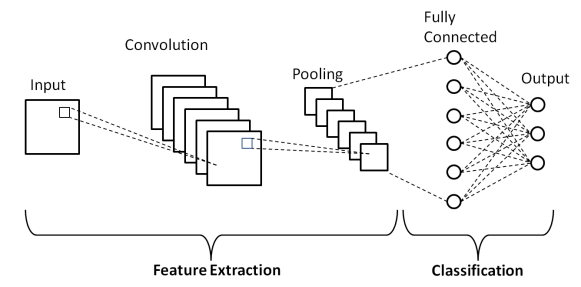
\includegraphics[width=1.0\textwidth]{CNN-architecture.png}
\caption{A basic convolutional neural network diagram}
\label{fig:CNN}
\end{figure}
\subsection{Learning solution data using autoencoders}
In this section, we will describe the deep autoencoder architecture and how the autoencode is used to learn the Boltzmann equation data solution and the Boltzmann collision operator. Figure \ref{fig:ae} shows a typical autoencoder architure. In an autoencoder, the number of neurons in an input layer is always equal to the number of neurons in the output layer. An autoencoder composes of two submodels: an encoder and a decoder.
\begin{figure}
\centering
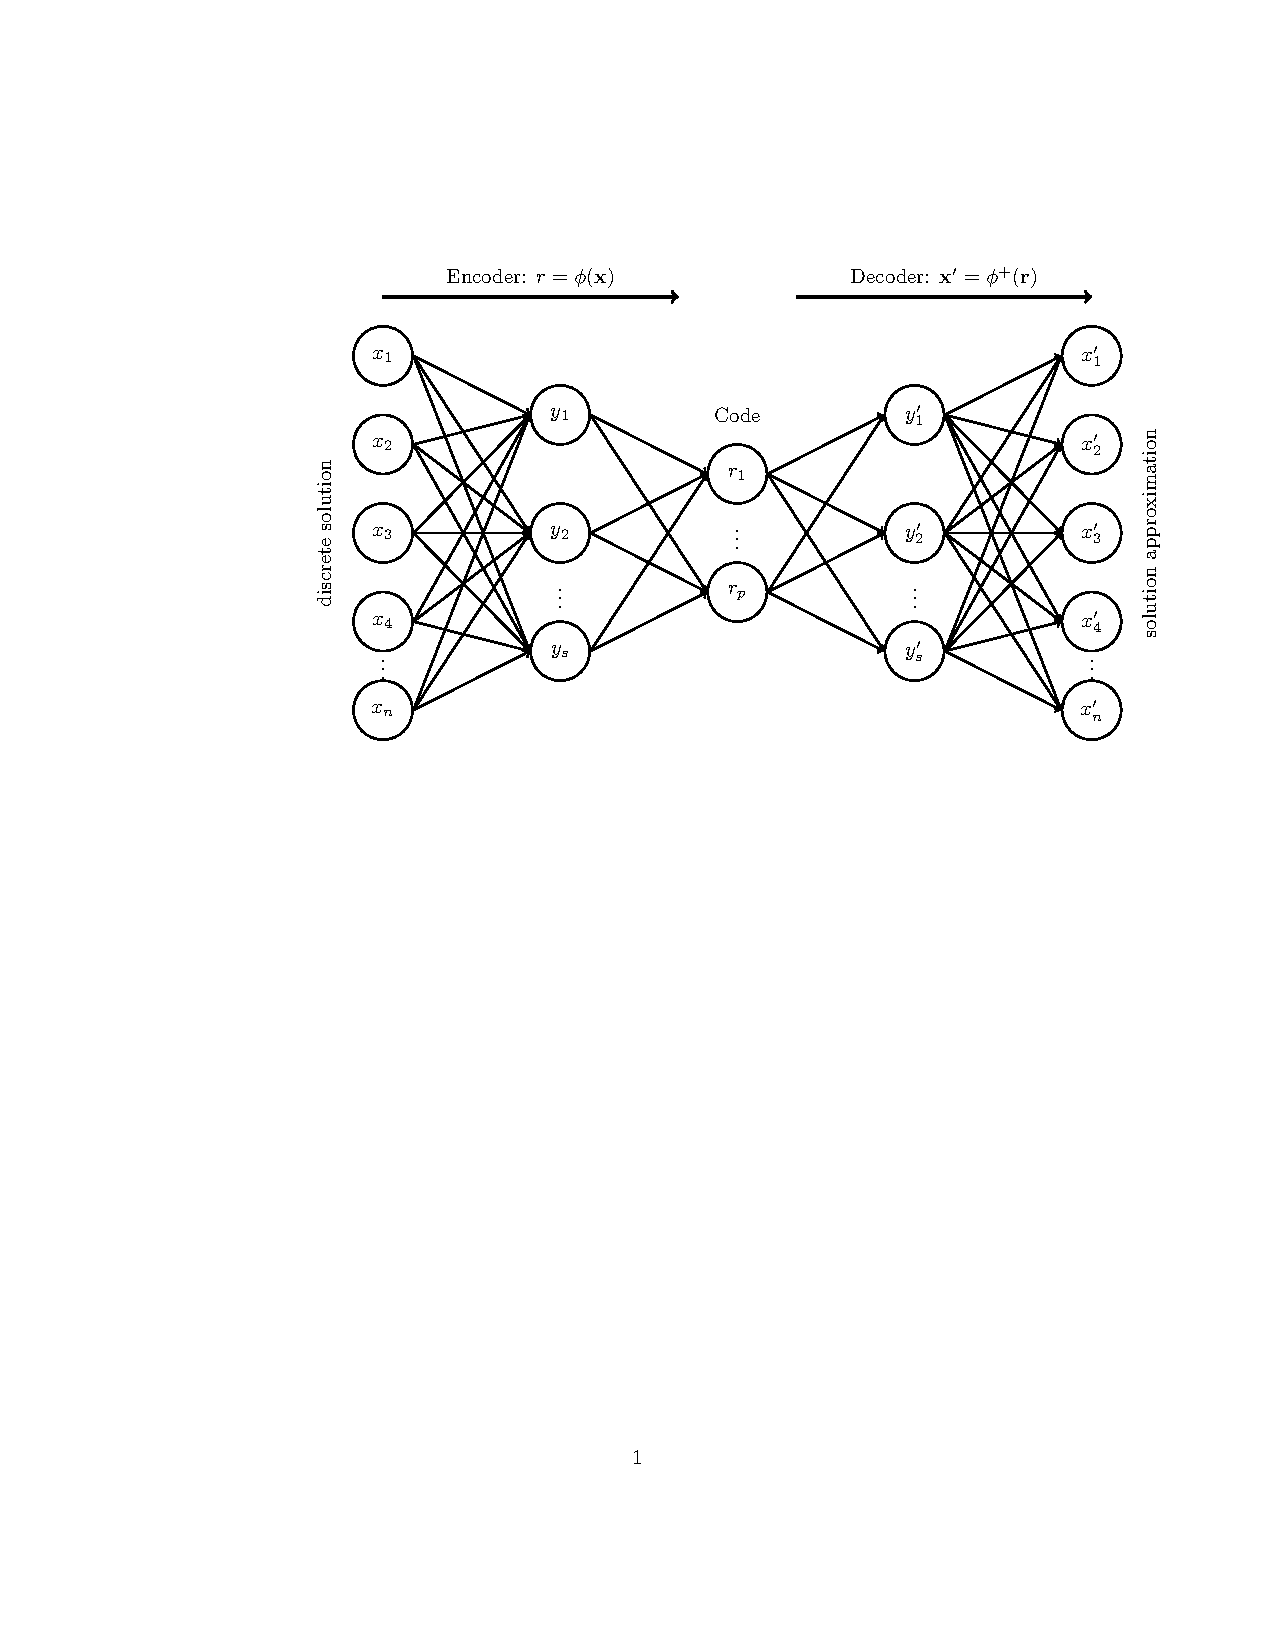
\includegraphics[width=1.0\textwidth]{Autoencoder.pdf}
\caption{A typical autoencoder architecture. An autoencoder composes of an encoder and a decoder. The encoder maps the input data to the code and the decoder reconstructs the inputs from the coding data}
\label{fig:ae}
\end{figure} 
The encoder model maps the inputs of higher dimension to a much lower dimensional data called the code. Then the coding data are fed into the decoder and the decoder reconstructs to output as the approximations of  inputs. The dimension of the code is much smaller than the dimension of the input. Autoencoder can be used to approximate the solutions of the Boltzmann equation as shown in the figure \ref{fig:ae}. The encoder $r = \phi()\mathbf{x})$ maps discrete solutions to the code. The code is the input of the decoder $\mathbf{x'}=\phi^+(\mathbf{r})$ and the output of the decoder is the approximation of the solution data.

We can also use autoencoder to learn the Boltzmann collision operator: $Q:\mathbb{R}^N\rightarrow\mathbb{R}^N$ which provides the derivatives of the velocity distribution
\begin{equation}
\partial_t{f(\vec{v})} = Q[f](\vec{v})
\end{equation}
As shown in figure \ref{fig:ColOpAE}, the Boltzmann collision operator is approximated by an autoencoder.
\begin{figure}[h]
	\centering
	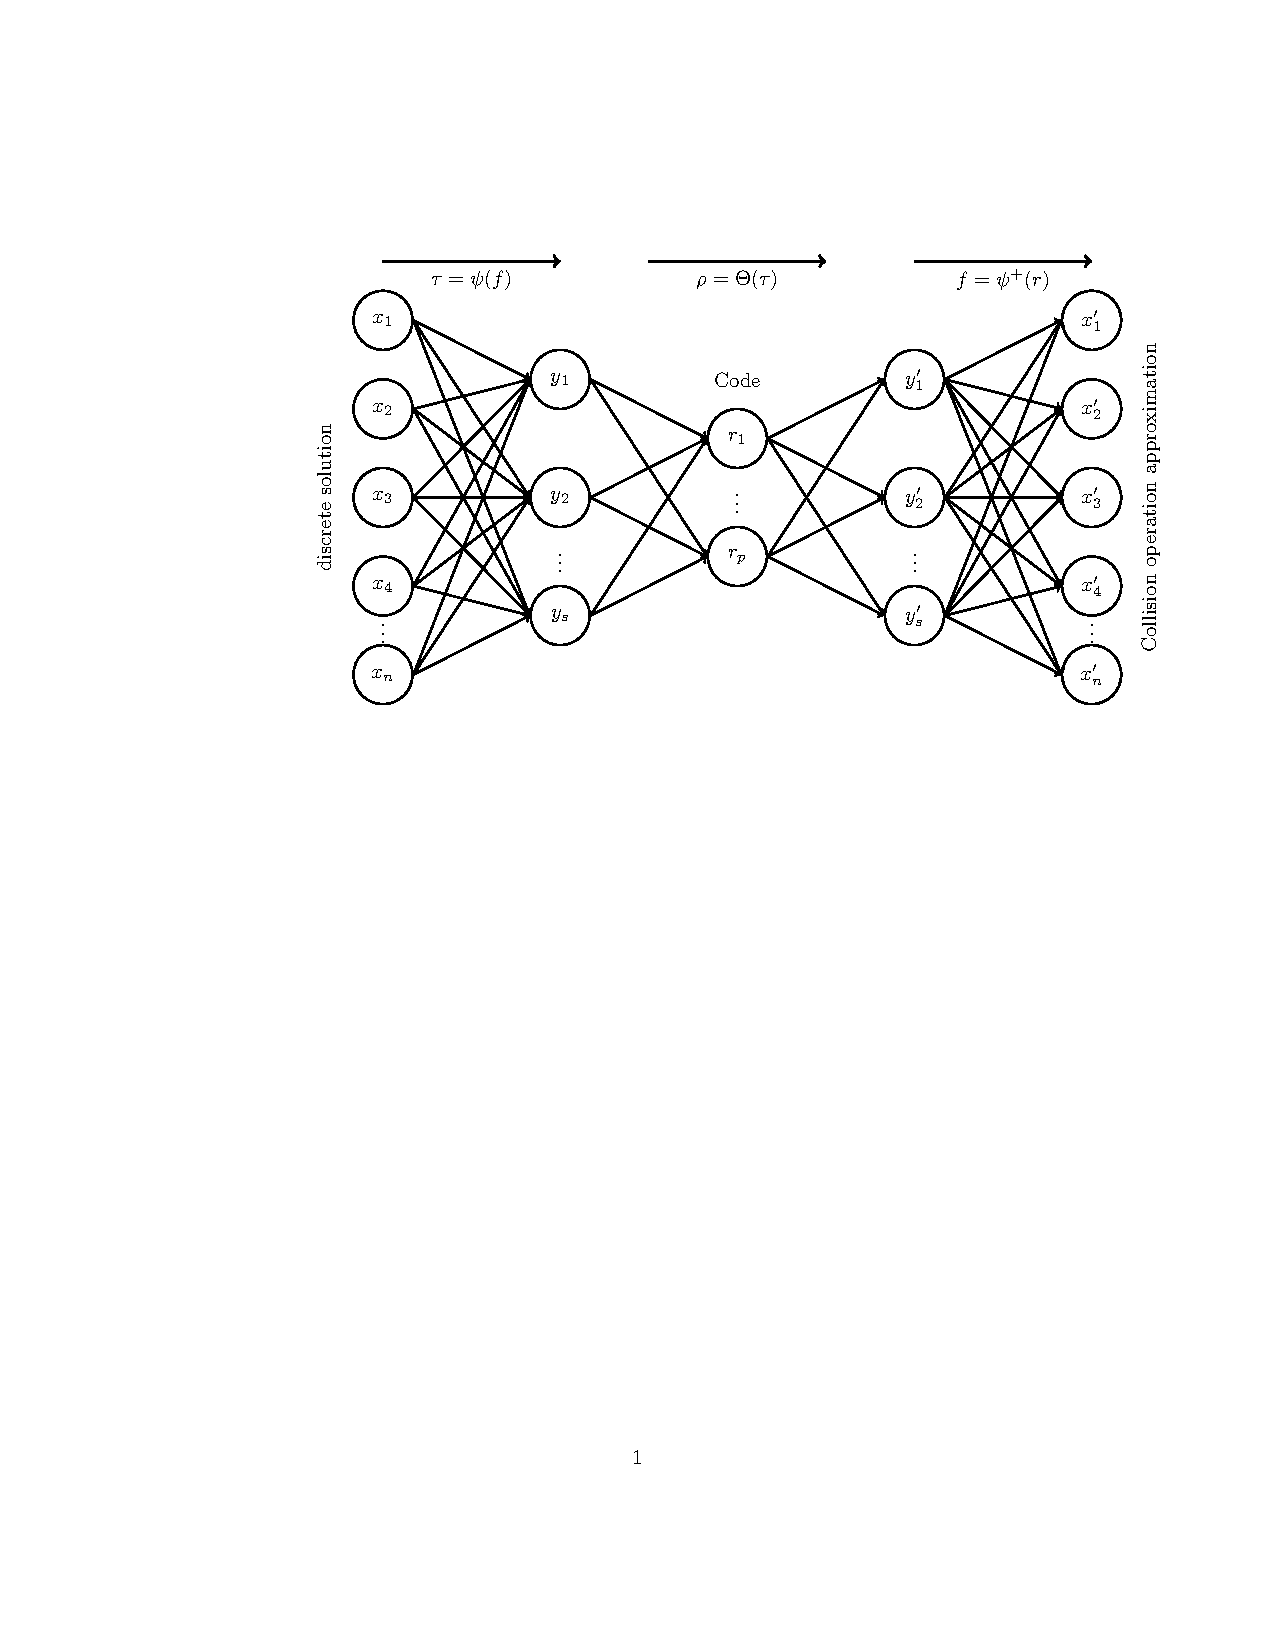
\includegraphics[width=.75\textwidth]{ColOpAE.pdf}
	\caption{An autoencoder that is used to approximate the Boltzmann collision operator}
	\label{fig:ColOpAE}
\end{figure}
\noindent To achieve fast evaluation, dimensions of the hidden layers should be significantly smaller than the size of input. Values predicted by the trained autoencoder can be used to approximate derivative of the solution and to do time integration. Formally, we can write
\begin{equation}
\partial_t{\tau} = \partial_t(\psi(f)) = \frac{\partial\psi}{\partial f}:\frac{\partial f}{\partial t} = \frac{\partial\psi}{\partial f}:Q(f) = \frac{\partial\psi}{\partial f}:Q(\psi^+(\tau)) = \phi(\tau)
\end{equation}

\subsubsection{Learing solution data using deep autoencoder}
In this section, we will discuss the results of using deep autoencoders to learn the Boltzmann equation solutions. One can refer to appendix A, appendix B, appendix C for the detail of how we used the software tools, language, and training environment to develop the different autoencoders. Table \ref{table:ae} below shows the accuracy of different deep autoencoders with various hidden layers and code lengths. Figure \ref{fig:lc} shows the learning curves of autoencoders with hidden layers of 1, 3, and 5 and code length of 32.

\begin{table} [h!]
\centering
\begin{tabular}{c|c|c|c|c|c|c|c|c|c}
	Hidden Layers & 1 & 1 & 1 & 3 & 3 & 3 & 5 & 5 & 5 \\
	\hline
	Code Length & 16 & 32 & 64 & 16 & 32 & 64 & 16 & 32 & 64 \\
	\hline
	Accuracy, MAE & 0.66 & 0.66 & 0.66 & 0.93 & 0.96 & 0.98 & 0.96 & 0.97 & 0.98
\end{tabular}
\caption{Accuracy of autoencoders with different number of hidden layers and code length. Mean absolute error (MAE) is used to measure the accuracy}
\label{table:ae}
\end{table}

\begin{figure}[h]
\begin{subfigure}{.5\textwidth}
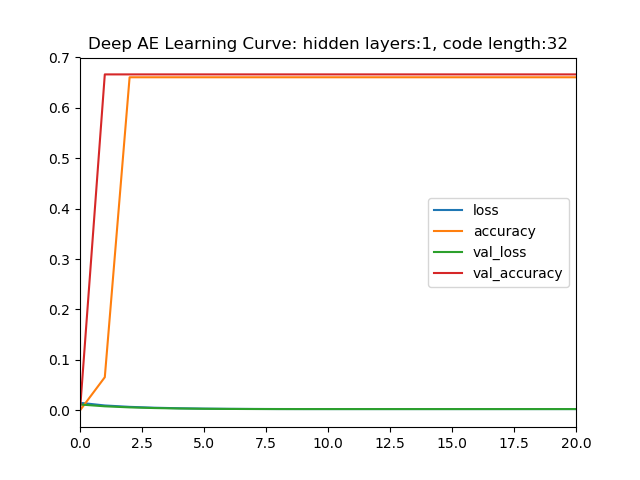
\includegraphics[width=.75\linewidth]{LearingCurve-HL1-CL32.png}
\end{subfigure}
\begin{subfigure}{.5\textwidth}
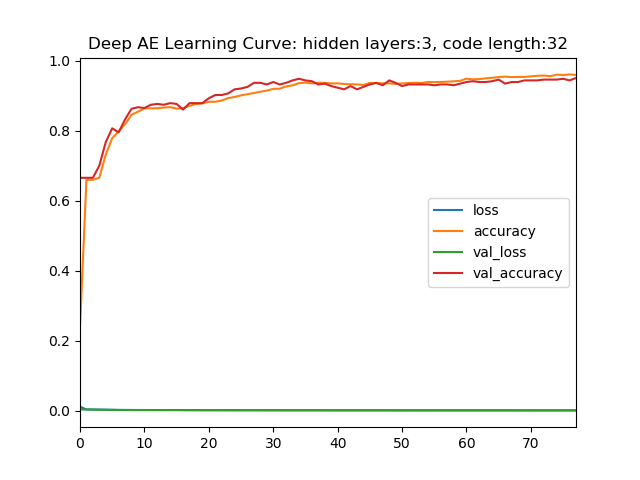
\includegraphics[width=.75\linewidth]{LearingCurve-HL3-CL32.png}
\end{subfigure}
\begin{subfigure}{.5\textwidth}
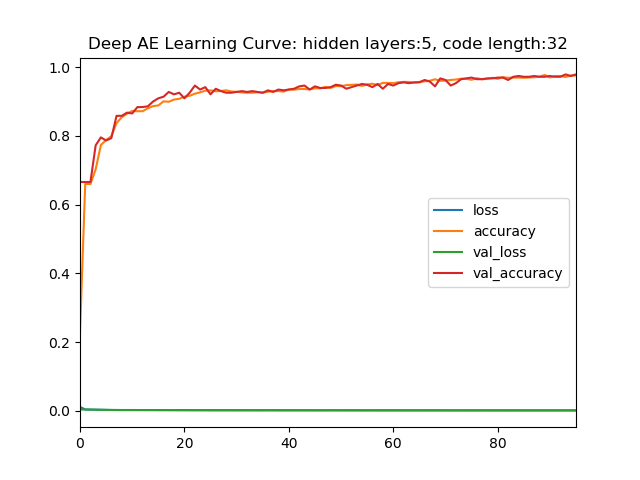
\includegraphics[width=.75\linewidth]{LearingCurve-HL5-CL32.png}
\end{subfigure}
\caption{Learning curves of autoencoders with hiddend layers of 1, 3, 5 and code length 32 }
\label{fig:lc}
\end{figure}
\noindent From \ref{table:ae} and \ref{fig:lc}, we have the following observations:
\begin{itemize}
	\item For autoencoders which have one hidden layer, the accuracy scores are low: 0.66. In this case, these autoencoders are underfitting.
	\item For autoencoders which have three hidden layers, the accuracy scores are very good. However, with code length of 64, the accuracy score is 0.98. In this case, the model could be overfitting.
	\item For autoencoders which have five hidden layers, the accuracy scores improve slightly comparing with the autoencodes with three hidden layers. 
\end{itemize}
Among these autoencoders, the autoencode with three hidden layers and code length 32 is probably is the best choice model. The second choice is the autoencoder with three hidden layers and code length 16 because the model is less complex, faster to train and compute, and the accuracy score is still about 0.93.

\subsubsection{Learing solution data using convolutional autoencoder}

\section{Computational efficiency comparisons between the numerial and neural network methods for computing the solutions of Boltzmann equation } \label{Comparisons}

\section{Conclusion} \label{Conclusion}

\appendix
\appendixpage
\section{Software language and tools for developing autoencoders}
Below are the software tools and language that we used to develop the autoencoders:
\begin{itemize}
	\item Computer language: Python 3.7.
	\item Neural networks development tools: Scikit-Learn, Keras, and Tensorflow.
	\item IDE development environment: VisualCode.
\end{itemize}
For code development, we use laptop/PC to develop the code, test and train autoencoders with solution data for only small number of iterations (or epoches) to ensure the code is working properly. Figures \ref{fig:settings}, \ref{fig:trainging}, and \ref{fig:training-results} shows how certain essential parmeters can be set by a setting file, the training accuracy in each epoch, and a directory that is used to save the training results.
\begin{figure}[h!]
	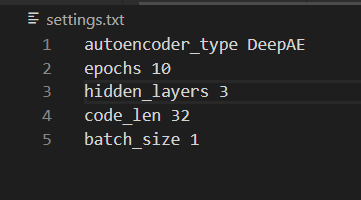
\includegraphics[width=.75\linewidth]{settings.png}
	\caption{This setting file is for the user to change important parameters for training different autoencoders}
	\label{fig:settings}
\end{figure}
\begin{figure}[h!]
	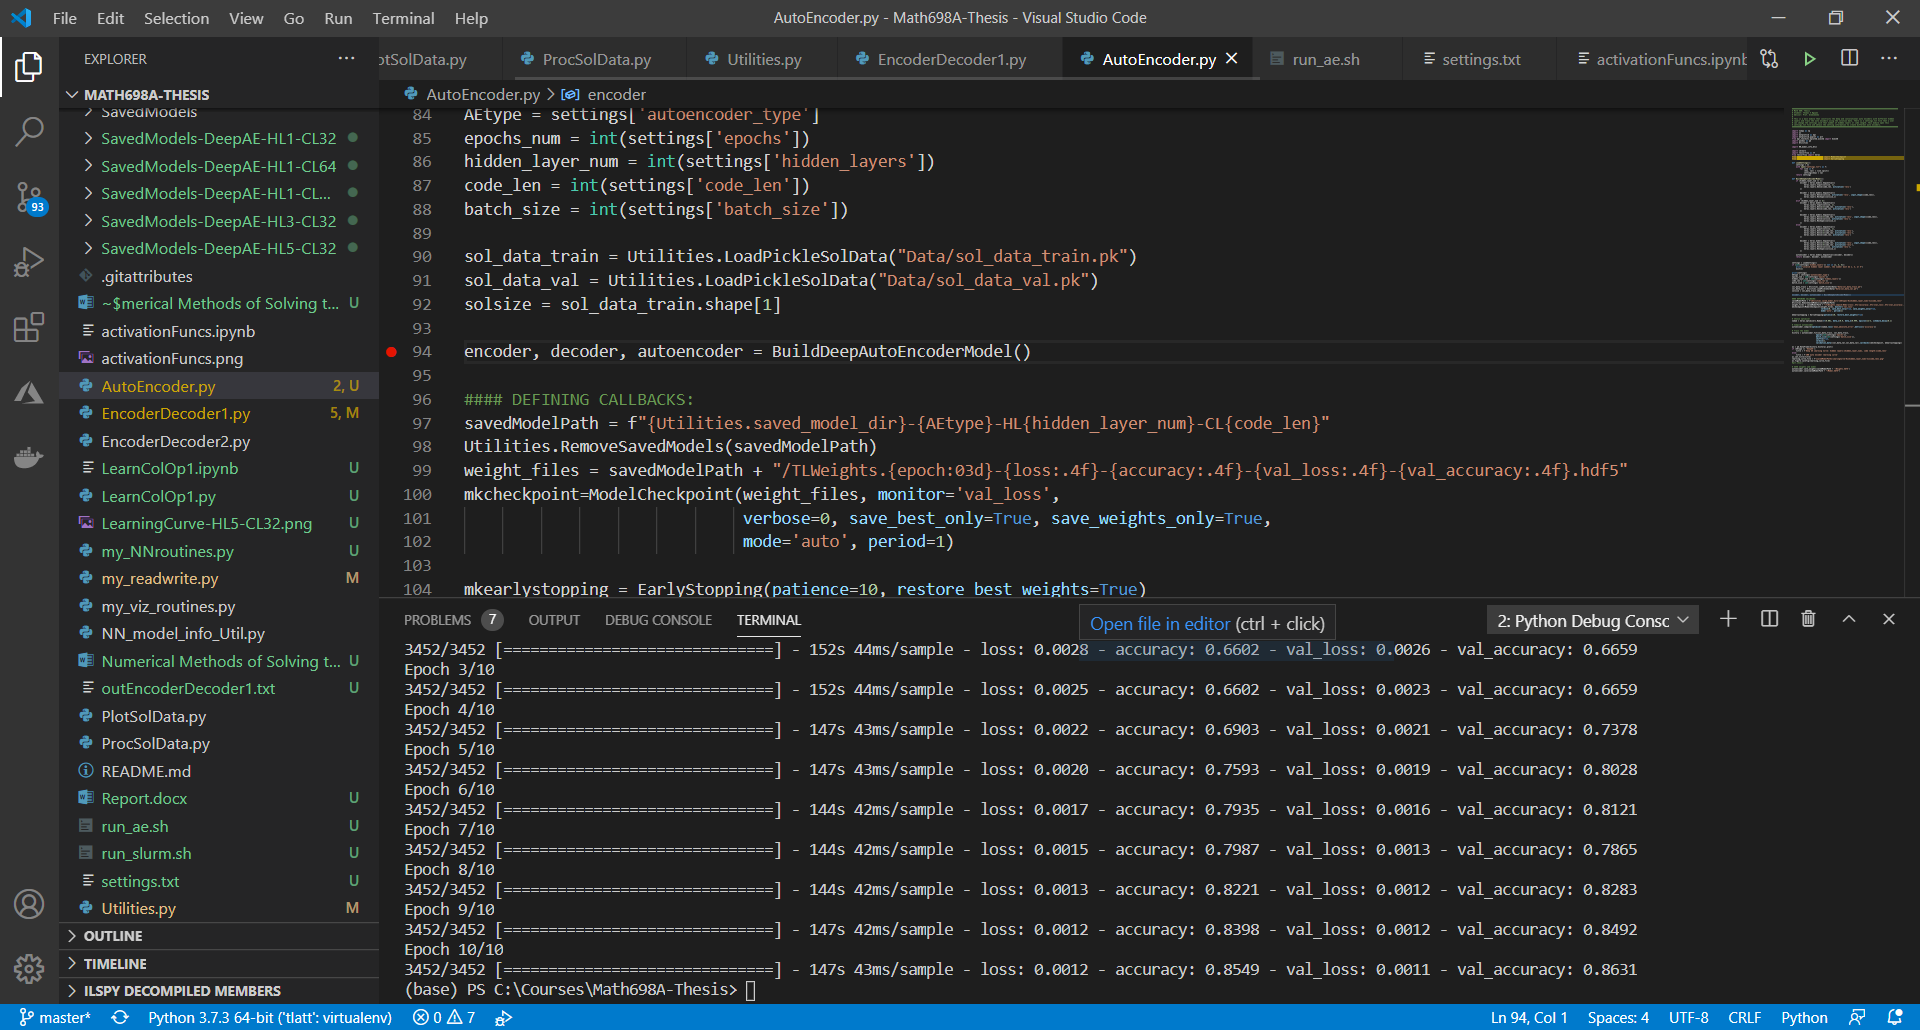
\includegraphics[width=1\linewidth]{training.png}
	\caption{Traing an autoencoder with three hidden layers, 10 epochs, code length=32}
	\label{fig:trainging}
\end{figure}
\begin{figure}[h!]
	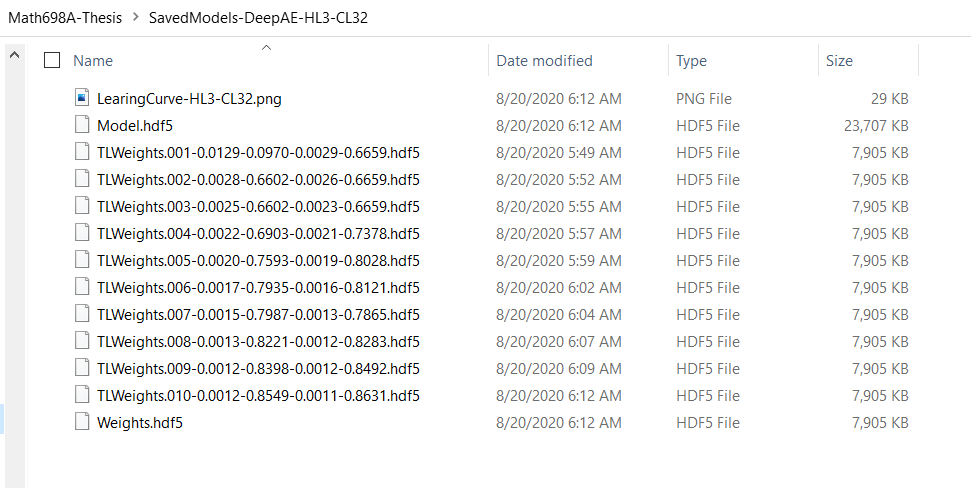
\includegraphics[width=1\linewidth]{training-results.png}
	\caption{This figure shows the training results that are saved in a directory. During the training, intermediate results are saved for each epoch. When the training completes, the learning curve plot is saved.}
	\label{fig:training-results}
\end{figure} 

Because training autoencoders can take several hours and computer resources, after testing the code working properly, we transfer python code and dataset to the XSEDE supercomputer to fully train and test our autoencoders as we describe in the next section.

\section{Testing and training autoencoder environments} 
After developed, tested, and trained the autoencoders on local computer, for fully training the autoencoders with the solution data, we need to connect to the XSEDE supercomputer system to train the autoencoders. Below are steps of how to we transfer the code and solution dataset to the XSEDE system to train the autoencoders. One can refer to document "StepsAccessToHPC.docx" written by professor Alekseenko for the detail of how to setup an XSEDE account, install PuTTY, FileZilla, etc. to connect to the XSEDE systems:
\begin{enumerate}
	\item Using PuTTY tool to establish remote connection to the XSEDE system as shown in figure \ref{fig:PuTTY}.
	\item Using FileZilla tool to connect to the XSEDE system and upload the python source codes, setting file, and solution dataset to a workspace directory on XSEDE under the home directory as show in figure \ref{fig:FileZilla}.
	\item Need to install Python, TensorFlow, Scikit-Learn if they are not installed on the working directory.
	\item Submit a batch file to XSEDE sytem to execute python code to train an autoencoder.
	\item After the training completed, all the results and plots are save to a appropriate directory so that we can download these files to the local computer via FileZilla tool.
	\item To train another autoencoders, change the number of hidden layers, and code length in the setting file and submit the batch file to the XSEDE system to execute the code.
\end{enumerate}
\begin{figure}[h!]
	\centering
	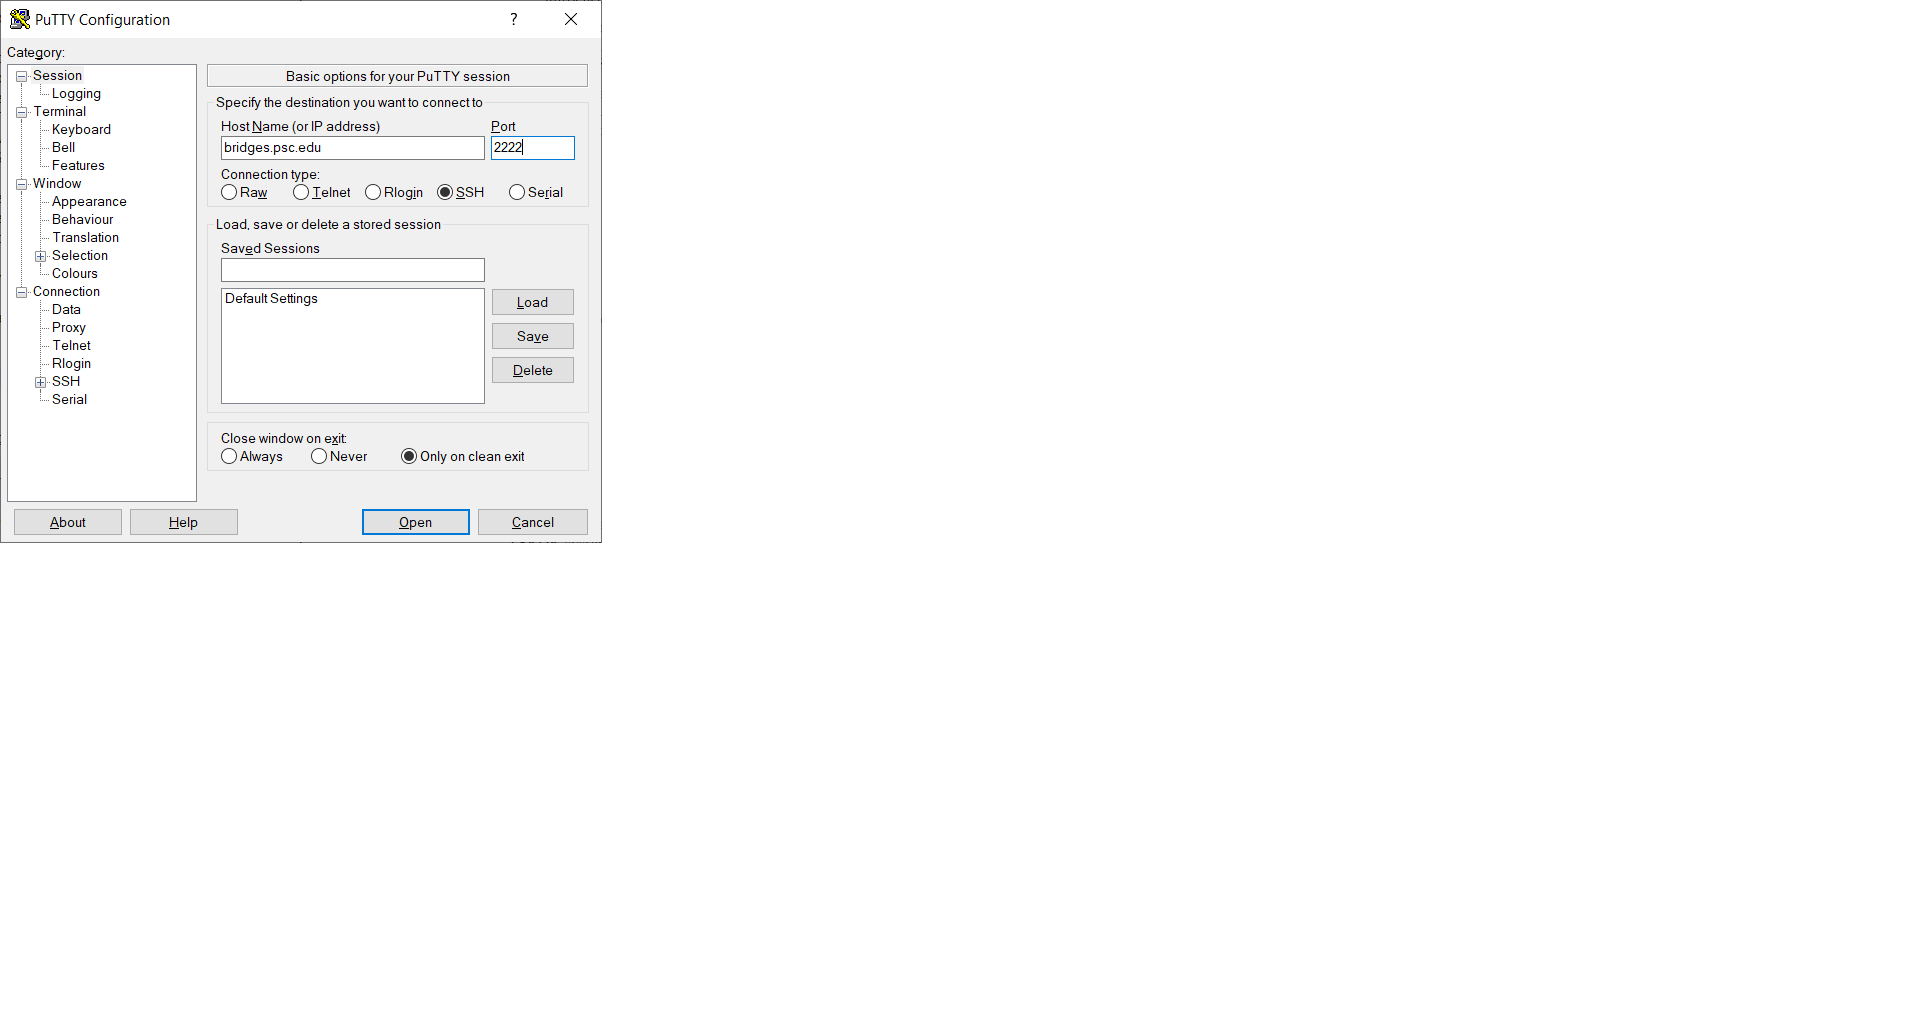
\includegraphics[width=1\textwidth]{PuTTY.png}
	\caption{Using PuTTY tool to connect to the XSEDE system }
	\label{fig:PuTTY}
\end{figure}
\begin{figure}[h!]
	\centering
	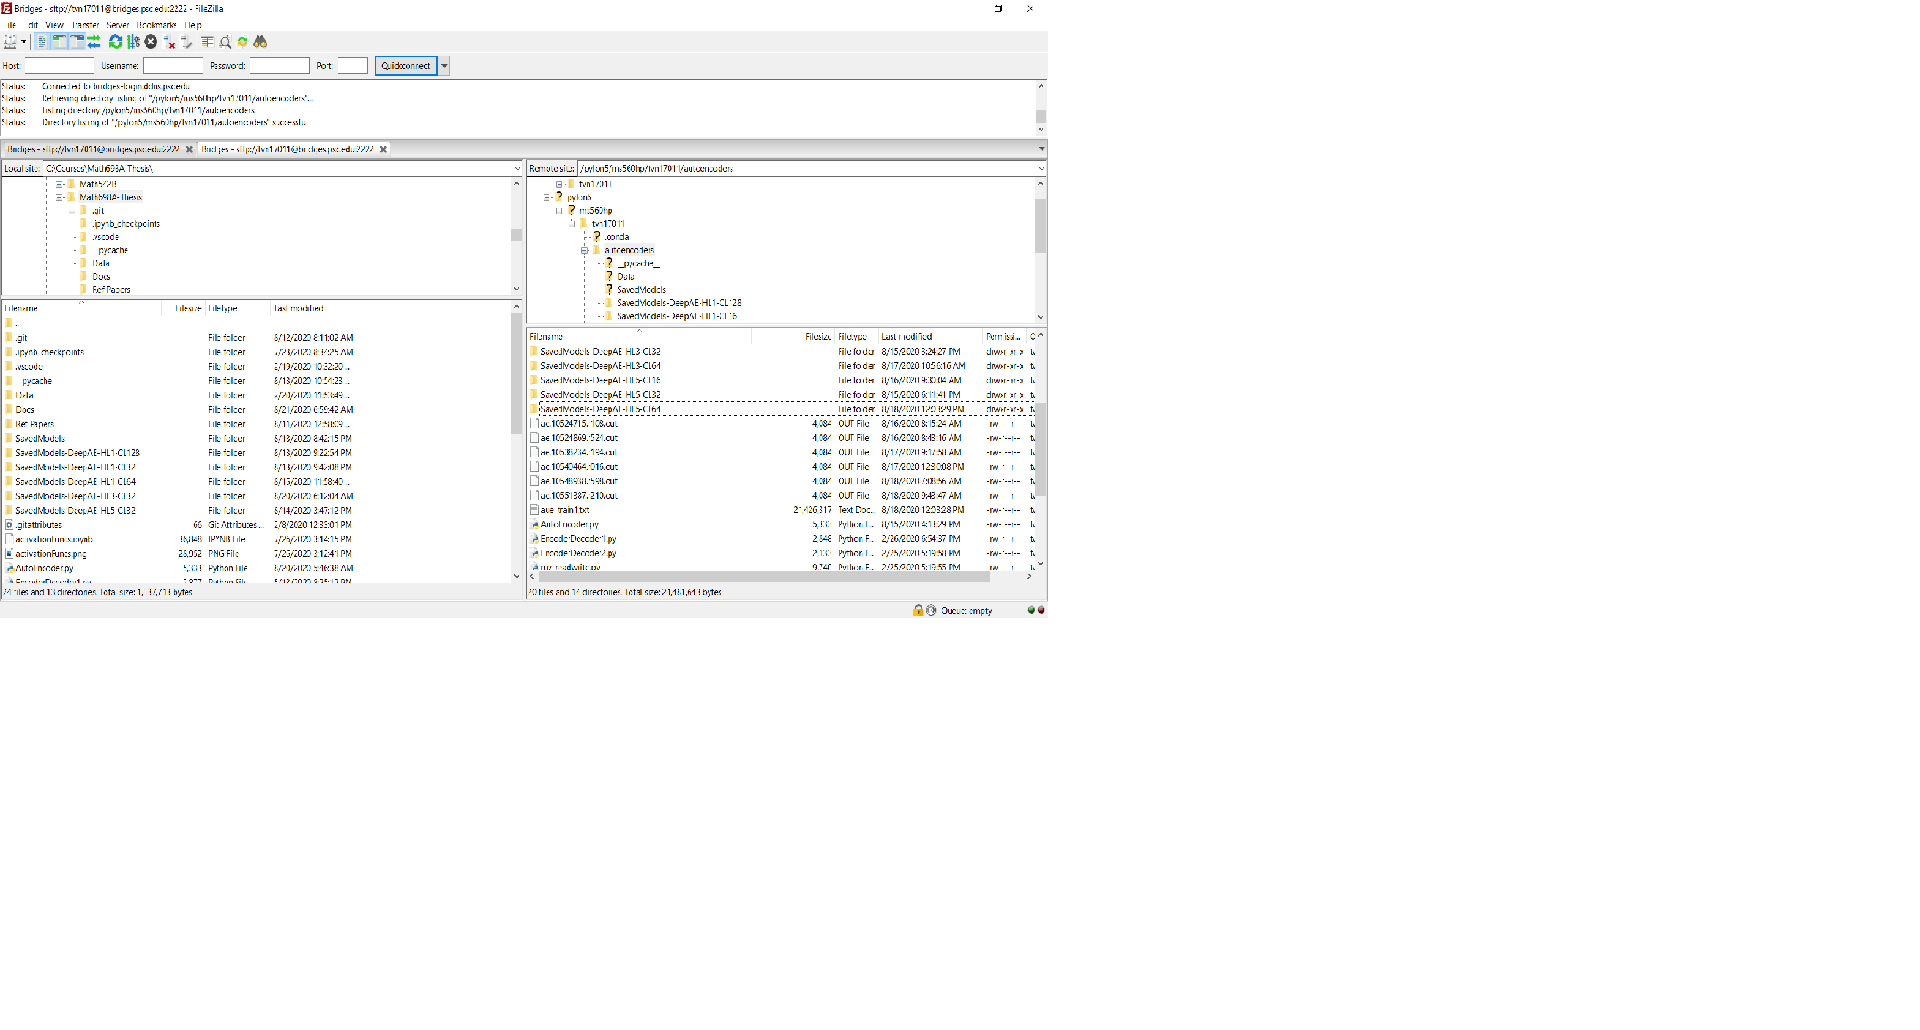
\includegraphics[width=1\textwidth]{FileZilla.png}
	\caption{Using FileZilla tool to upload or download files to the XSEDE system.}
	\label{fig:FileZilla}
\end{figure}
Typically, when we train an autoencoder with 100 epoches (iterations) on the XSEDE system, it takes less than an hour while it takes several hours and sometimes the computer crashed when training an autoencoder with 50 epoches on our PC.
\section{Documents and source code revision control}
We maintain source files, documents, and revisions in GitHub under \\ \href{https://github.com/tlatttt/Math698A-Thesis}{https://github.com/tlatttt/Math698A-Thesis}. Figure \ref{fig:GitHub} shows the source files and directories of this project on the GibHub. 
\begin{figure}[h!]
	\centering
	\includegraphics[width=1\textwidth]{GitHub.png}
	\caption{A screen shot of the source files, documents that are maintained on GitHub}
	\label{fig:GitHub}
\end{figure}
Below are the important source files and directories for this project:
\begin{itemize}
	\item  \textit{AutoEncoder.py} is the main module responsible to create deep and CNN autoencoders, perform the training, and save the models and accuracy scores.
	\item \textit{Settings.txt} is the text file for changing the parameters for autoencoders such as number of epoch, number of hidden layers, etc.
	\item \textit{Utilities.py} is a module that provides utility functions for other modules. \textit{AutoEncoder.py} calls a function in this module to delete the previous trained results in a directory before training an autoencoder so that the new trained results can be saved in this directory.
	\item \textit{Data} is a directory that contains the training and validation files used to train the autoencoders.
	\item \textit{Docs} is a directory contains documents  this project. This directory also contains LaTex source files that are used to generate the PDF document files.
	\item \textit{Ref Papers} contains all the reference papers for the thesis report.	
\end{itemize}
\pagebreak
\begin{thebibliography}{99}
	\bibitem{RarefiedGasD}M. Kogan, Rarefied gas dynamics, Plenum Press, 1969.
	\bibitem{IntroBoltz}Stewart Harris, An Introduction to the Theory of the Boltzmann Equation, 1971, 2004.
	\bibitem{Alekseenko1}A. Alekseenko and E. Josyula.  Deterministic Solution of the Boltzmann Equation Using a Discontinuous Galerkin Velocity Discretization. In 28th, International Symposium on Rarefied Gas Dynamics, 9-13 July 2012, Zaragoza, Spain, AIP Conferences Proceedings, page 8. American Institute of Physics, 2012.
	\bibitem{Alekseenko2}A. Alekseenko and E. Josyula.  Deterministic Solution Of The Spatially Homogeneous Boltzmann Equation Using Discontinuous Galerkin Discretizations In The Velocity Space. Journal of Computational Physics, 272(0): 170 – 188, 2014.
	\bibitem{Alekseenko3}A. Alekseenko, T. Nguyen, and A. Wood. A Deterministic-Stochastic Method For Computing The Boltzmann Collision Integral In O(Mn) Operations. Kinetic \& Related Models,11(1937-5093.2018.5.1211):1211, 2018.
	\bibitem{Alekseenko4}Alexander Alekseenko and Jeffrey Jimbacher. Evaluating High Order Discontinuous Galerkin Discretization of The Boltzmann Collision Integral In O(N2) Operations Using The Discrete Fourier Transform, 2019.
	\bibitem{LBM1} Peter Mora, Gabriele Morra and David A. Yuen. A concise python implementation of the lattic Boltzmann method on HPC for geo-fluid flow, Geophysical Journal International 2019.
	\bibitem{LBM2} Timm K\"{u}ger, Halim Kusumaatmaja, Alexandr Kuzmin, Orest Shardt, Goncalo Silva, and Erlend Magnus Viggen. The Lattic Boltzmann Method, Principles and Practice. Springer 2017
	\bibitem{WikiTheoryOfGas}Wikipedia, Kinetic theory of gases,https://en.wikipedia.org/wiki/Kinetic\_theory\_of\_gases.
	\bibitem{DSMC1}Fransis J. Alexender, Alejandro L. Garcia, The Direct Simulation Monte Carlo Method, Computer In Physics, Vol 11, Nov 1997.
	\bibitem{DSMC2}Lorenzo Pareschi, Giovanni Russo, An Introduction to Monte Carlo Methods for Boltzmann Equation, ESAIM Proceedings, 1999.
	\bibitem{DSMC3}A. A. Ganjaei and S. S. Nourazar, A new algorithm for the simulation of the boltzmann equation using the direct simulation monte-carlo method, Journal of Mechanical Science and Technology 23 (2009) 2861~2870.
	\bibitem{BirdGA1}Bird, G. A., “Approach to Translational Equilibrium in a Rigid Sphere Gas.” Physics of Fluids, Vol. 6, 1963, pp. 1518-1519.
	\bibitem{BirdGA2}Bird, G. A., Molecular Gas Dynamics and the Direct Simulation of Gas Flows, Charendon Press, Oxford, 1994.
	\bibitem{VVAristo} V. V. Aristo. Direct Methods for Solving the Boltzmann Equation and Study of Nonequilibrium flows, 2001.
	\bibitem{HandOnML}Anr\'{e}lien G\'{e}ron, Hands-on Machine Learning with Scikit-Learn, Keras \& TensorFlow, O'Reilley, 2019
	\bibitem{IntroML}Andreas C. Müller, Guido, Sarah. Introduction to Machine Learning with Python, 2017.
	\bibitem{DeepLearning}John D. Kelleher, Deep Learning, The MIT Press, 2019.
	\bibitem{Autoencoder1}Francois Chollet et al. Keras. https://github.com/fchollet/keras, 2015.
\end{thebibliography}
\end{document}